\chapter{Experiments}

All our reality gap approaches have been validated on a robotic application with the Thymio robot on an obstacle avoidance task. The experimental set up among all approaches mainly differ in the evolutionary strategy used or whether the optimization happened fully or partially in simulation and reality. The following next paragraphs describe the common set-up used in our experiments.

The robot is quipted with 7 infrared sensors and 2 two motors. The virtual thymio robot is modeled based on the physical thymio and its characteristics \ref{thymio_characteristics}. The specifications of sensor readings and possible speed values, included normalization values are depicted in the following table \ref{fig:thymio_specs} both for the physical thymio and its virtual counterpart.

\begin{table}[H]
\begin{tabular}{llll}
\centering
\hline
\textbf{}                            & \textbf{Simulator}    & \textbf{Reality}  & \textbf{Normalized}  \\ \hline
\textbf{Speed Values}                & {[}-2.0, 2.0{]}       & {[}-200, 200{]}      & {[}0.0, 1.0{]} \\
\textbf{Sensory Readings}            & {[}0.0, 1.0{]}        & {[}0, 4500{]}        & {[}0.0, 1.0{]} \\
\end{tabular}
\caption{The Thymio robot sensors and speed values specification.}
\label{tab:thymio_specs}
\end{table}

The evaluation of a single genome takes 60 simulation seconds for the simulation-based approaches and 60 wall clock seconds for the reality-based approaches from a fixed initial position each test. At each step (50ms), the Thymio robot sensory readings are fed to the neural network and the network outputs are multiplied by the maximal wheel speed and used to apply to the wheels of the Thymio robot. The network outputs are in the range of \emph{0.0} and \emph{1.0}, and since the Thymio can move backward, the output values are transformed into a positive/negative range where \emph{0.5} is the point of direction inversion. In order to speed up the optimization, the evaluation of a genome is stopped if the system detects that the robot collided with the walls or the environmental objects. Furthermore, if the robot is not moving or spinning in one place the evaluation is stopped and the fitness is calculated over reduced simulation time.

The fitness function relies on a set of features that can be measured within the interaction between the robot and its environment. Hence the fitness function relies on 3 features, as follows:

\begin{enumerate}
    \item \(V_{t} = \frac{V_{l} + V_{}r}{2} \) \textbf{Average wheel speed} of both wheels at a particular timestamp \emph{t}.
	\item \((1-\sqrt{\Delta v})\) \textbf{The algebraic difference} between the speed values at a particular timestamp \emph{t}. The smaller is the difference, the faster the robot moves.
	\item \((1 - P_{t})\) \textbf{Max Sensor activation} the activation value of the proximity sensor with the highest activity. The closer the robot is to the walls or obstacles the less fitness it accumulates.
\end{enumerate}

The fitness function \ref{eq:fitness_function} is defined as a dot product of all these features divided by the fixed simulation time. 

\begin{equation}
	f = \sum_{t=1}^{t_{max}} \frac{V_{t} (1 - \sqrt{\Delta v}) (1 - P_{t})}{60}
	\caption{Task dependent fitness function}
	\label{eq:fitness_function}
\end{equation}

For each evaluated controller, we extract certain \emph{behavioral feautures} \ref{eq:behavioral_features} during the optimization process. These features allow us to describe/quantify the behavior of each controller. Moreover, it allows us to compare controllers in a simple manner without any dependency on the evolutionary strategy applied or the controller's genotype. The 12-dimensional features are defined as 1) the average left and right wheel speeds 2) the average value of each sensor activation 3) percentage of time spent in each section of the arena throughout the evaluation. These features are normalized in the range of \emph{0.0} and \emph{1.0}.

\begin{equation}
	b_{controller} = [avg_{left}, avg_{right}, s_{1}, s_{2}, s_{3}, s_{4}, s_{5}, s_{6}, s_{7}, area_{0}, area_{1}, area_{2}]
	\caption{12-dimensional behavarioral features}
	\label{eq:behavioral_features}
\end{equation}

Additionally, we extract the position of the Thymio robot during evaluation. The vision system is used to extract the position from reality and the system is responsible for the position from the simulation. This feature measure is used to qualify a given controllers transfer from simulation to reality.

\section{Simulation-based optimization}

Our first application aims to explore the \emph{simulation-based optimization} approach to the reality gap problem. The first part of the experiments involves evolving an obstacle avoidance behavior in simulation. Finding the right parameters of the evolutionary strategy to achieve optimal obstacle avoidance behavior, like, number of generations, population number, etc. The second part is focused on the transferability of controllers. Taking the best controllers evolved in simulation and validate how well they transfer to reality. Additionally, this approach is later compared to the reality-based optimization approach to the same application.

\subsection{Experimenal design}

The first experiment takes place fully in simulation using the simulation model mentioned earlier \ref{fig:virtual_arena}. The aforementioned evolutionary algorithm applied in this experiment is \emph{NEAT} \citep{stanley2002evolving}. A controller, in this case, the genome, is represented as a neural network. The implementation is based on the python-neat \footnote{\url{https://neat-python.readthedocs.io/en/latest/}} library which has been modified to fit our requirements. The genome contains a list of \emph{connection genes} and list of \emph{node genes}. Node genes encode the input, hidden nodes, and outputs of the neural network that can be connected. Whether a node is connected to other node is expressed in the connection gene. The initial neural network structure consists of 7 input nodes (each represents the infrared sensors placed around the Thymio), fully connected to the 2 motor neurons computing the speeds of the wheels. This way the algorithm starts with a fixed topology and by applying the biological operators over generations it may evolve. In the early stage of the experiments various parameters of the evolution have been tested (population size, generations, mutation rate, etc.), but the most promising results have been achieved by the parameters summarized in table \ref{tab:neat_parameters}. The experiment have been reproduced 10 times.

\begin{table}[H]
\centering
\begin{tabular}{ll}
\hline
\textbf{}                      & \textbf{} \\ \hline
\textbf{Population size}       & 20        \\
\textbf{Number of generations} & 20        \\
\textbf{Simulation time}       & 60 sec    \\
\textbf{Activation function}             & sigmoid       \\
\textbf{Connection add probability}              & 0.5       \\
\textbf{Connection delete probability}              & 0.5       \\
\textbf{Node add probability}              & 0.2       \\
\textbf{Node delete probability}              & 0.2       \\
\textbf{Elitism}  & 1      
\end{tabular}
\caption{Parameters of the NEAT algorithm.}
\label{tab:neat_parameters}
\end{table}

\section{Reality-based optimization}

\subsection{Experimenal design}

For comparison to the simulation-based optimization, we conduct a reality-based optimization directly on the physical robot. The experimental set-up is the same as in the previous application. The size of the population is 20 and the number of generations is 20. Again, NEAT is used as the underlying evolutionary strategy with the same parameters summarized in table \ref{neat_parameters}. It has been reproduced 10 times, which implies 4000 evaluations, to have the same amount of experiments in reality as in simulation. The experiment completely relies on the entire robotic platform including the vision system, simulation, and the Thymio robot.

\section{Transferability Approach}.

This series of experiments falls into the \emph{robot-in-the-loop simulation-based optimization}. Our aim is to validate the transferability approach to obstacle avoidance task based on \citep{koos2012transferability}. We assume that more transfers from simulation to reality allow to approximate the surrogate model better which could guide the evolutionary search to more transferable controllers.

\subsection{Experimenal design}

The transferability approach relies on a multi-objective formulation of the evolutionary strategy where the two main objectives are optimized with Pareto-based ranking scheme. Our implementation relies on the \citep{deb200fast} evolutionary algorithm implemented via the \emph{DEAP}\footnote{\url{https://deap.readthedocs.io/en/master/}} library. Each controller is evaluated by three objectives:

\begin{enumerate}
	\item the \emph{task-dependent fitness}\ref{eq:fitness_function}, to find controllers with obstacle avoidance behavior. 	The algorithm maximizes this objective.
	\item the corresponding \emph{simulation-to-reality disparity} (STR disparity), which is minimized, to find optimal transferable controllers.
	\item the \emph{behavioral diversity} objective, which is maximized, to find more diverse set controllers.
\end{enumerate}

\emph{STR disparity and the surrogate model}. The transferability of a given controller is evaluated by the  STR disparity measure \(D^{*}_{{c}}\), which directly quantify the behavioral disparities between any possible controller observed in simulation and in reality. The same STR disparity measure is used in our experiment as in the original implementation. Its computed as the mean square error between the corresponding trajectories between simulation and in reality during evaluation. The exact STR disparity \(D^{*}_{{c}}\) of a controller is defined as:

\begin{equation}
	D^{*}_{{c}} = \sum_{t=1}^{t_{max}} \frac{(x^{i}_{S} - x^{i}_{R})^{2}}{\bar{x_{S}}\bar{x_{R}}} + 							  \sum_{t=1}^{t_{max}} \frac{(y^{i}_{S} - y^{i}_{R})^{2}}{\bar{y_{S}}\bar{y_{R}}}
	\label{eq:The exact STR disparity measure.}
\end{equation}

Where $ S_{t_{max}} = \{{x_{S}, y_{S}} \}$  and $ R_{t_{max}} = \{ {x_{R}, y_{R}} \} $ is a set of positions extracted in simulation and reality, $ \bar{x_{S}} $ (resp. $ \bar{y_{S}}, \bar{x_{R}}, \bar{y_{R}} $) is the mean of $ x^{t_{max}}_{S} $ (resp. $ y^{t_{max}}_{S}, x^{t_{max}}_{R}, x^{t_{max}}_{R} $). The exact STR disparity measure cannot be used directly for the optimization scheme for each controller, because it would require to transfer each controller during the evaluation, therefore the approach relies on a so called \emph{surrogate model} which approximates this measure. The surrogate model is approximated by Inverse Distance Weightining interpolation method \citep{shepard1968two}. The \emph{surrogate model of the STR disparity} is defined:

\begin{equation}
	
	\[ \forall{c}\in\chi, \hat{D}_{(c)} = \frac{\sum_{c_i\in\chi_T} {D^{*}_{(c)} b_{dist}(c_{i}, c)^{-2}}}
										{\sum_{c_i\in\chi_T} {b_{dist}(c_{i}, c)^{-2} }} \]
	\label{eq:surrogate_model}
\end{equation}

Where $\chi$ is the set of all controllers in the population, $\chi_T \subset \chi$ is the set of the already transferred controllers and $D^{*}_{(c)}$ is the exact STR disparity value corresponding to each controller $c_i \in \chi_T$.

The last evaluation objective of the optmization scheme is the \emph{behavioral diversity}, which quantify the diversity of a controller from the already transfered ones. For a given controller the diversity $ diversity_{(c)}$ is:

\begin{equation}
	diversity = \min_{\forall c_i \in \chi_T } b_{dist}(c, c_i)
	\label{eq:behavioral_diversity}
\end{equation}

$b_{dist}$ is the euclidean distance between the \emph{12th} dimensional behavioral features\ref{eq:behavioral_features}.

For this approach we use a feed-forward neural network with static structure. The network is fully connected, containing 7 input neurons, 1 hidden layer with 14 neurons, and 2 motor neurons calculating the wheel speeds. The activation function is the same as in the previous experiments. In this case the genome encodes the weights of the neural network as a vector of floating point values. All genomes are bound to two genetic operators. Two point crossover is applied with probability 0.5 and a gaussian mutation with probability 0.7 mutating each attribute of the genome. The experimental configuration can be seen in table \ref{tab:moea_parameters}

\begin{table}[H]
\begin{tabular}{ll}
\hline
\textbf{}                      & \textbf{} \\ \hline
\textbf{Population Size}       & 80        \\
\textbf{Number of Generations} & 40        \\
\textbf{Simulation time}       & 40 sec    \\
\textbf{Crossover}             & 0.2       \\
\textbf{Mutation}              & 0.1       \\
\textbf{Tournament Selection}  & 3        
\end{tabular}
\caption{Parameters of the Multi-objective optmization procedure.}
\label{tab:moea_parameters}
\end{table}


\emph{Algorithm outline}. The multiobjective evolutionary strategy starts by initialzing the surrogate model of the STR disparity function by randomly selecting a $c_{(0)}$ controller among the first population. The $c_{(0)}$ controller is evaluated in simulation and then transfered to reality. The corresponding STR disparity $ D^{*}_{(c_0)}$ value, behavioral features are obtained and the surrogate model is computed/initialized. Afterwards, each generation of the algorithm follows as:

\begin{description}
	\item[1. Evaluation] of each controller
		\begin{description}
			\item[STEP 1] Computation of the task-dependent fitness, behavioral features in simulation. Respectively, aggregating the path traveled.
			\item[STEP 2] Evaluation of the approximated STR disparity (surrogate model) and behavioral diversity, based on the already transfered controllers.
		\end{description}
	\item[2. Transferability selection] 
		\begin{description}
			\item[STEP 1] Controllers with high enough diversity are selected from the current population and transferred to reality.
			\item[STEP 2] Computation of the exact STR disparity measure between the simulation and reality. Updating the surrogate model based on obtained results.
		\end{description}
	\item[3. Genetic Operators] Application of the genetic operators (crossover & mutation)
\end{description}


\subsection{Complications of the implementation and the experiments.} 

In order order to obtain controllers that transfer well from simulation to reality we tried to implement the original implementation with all its perks. Nevertheless, we have discovered/encountered the following issues:

\begin{description}
	
    \item{STR Disparity Measure}. In the initial experiments, we have defined the exact STR disparity measure as the Euclidean distance between the corresponding trajectories observed in simulation and in reality. It has been changed to the mean square error from the original implementation, which also turned out to evaluate more accurately the error between simulated and real trajectories. As it can be seen on a sample \ref{fig:trajectory_discrepancy}, the traveled discrepancies between simulation and reality computed with the Euclidean distance is \textit{1.958}, on the other hand, the discrepancy computed with the mean squared error is \textit{26.596}. This turned out to be problematic when comparing trajectories that are highly diverse, which resulted in a badly modeled surrogate model. Relying on the mean square error had the benefit of penalizing large errors more, which was appropriate to accurately model the surrogate model. 
    
    \item{Calculation of the exact Disparity Measure}. As one can assume from figure \ref{fig:trajectory_discrepancy}, it is clear that the Thymio (transferred controller in reality) behaves differently than its counterpart in simulation. In simulation the robot is keep facing the wall and stay still the rest of the simulation time, on the other hand the transfered controller goes straing until it hits the obstacle, this is the result of a reality gap. In consequence with our initial constraints of measuring the disparity lead to inaccurate results of the exact disparity between simulation and reality, likewise inaccurate surrogate model. Since our implementation was concerned of taking always the N-M (or vice versa) size of \[ [(x_1,y_1), (x_2, y_2), ...] \] coordinate samples both from simulation/reality, thus calculating the mean square error based on only N-M samples. It notably means that the exact str disparity measure is over-fitting, therefore not sufficient to describe the disparities. Furthermore, the collision detection was also applied for the transferred controllers, which also skewed the values. This miscalculation is depicted in figure \ref{fig:trajectory_discrepancy_wrong_measure}. To cope with these potential miscalculations, this constraint was removed and later on the entire trajectory is used to correctly calculate the exact STR disparity.
	
\end{description}

\begin{figure}[H]
    \centering
    \begin{subfigure}[b]{0.8\textwidth}
    	\centering
        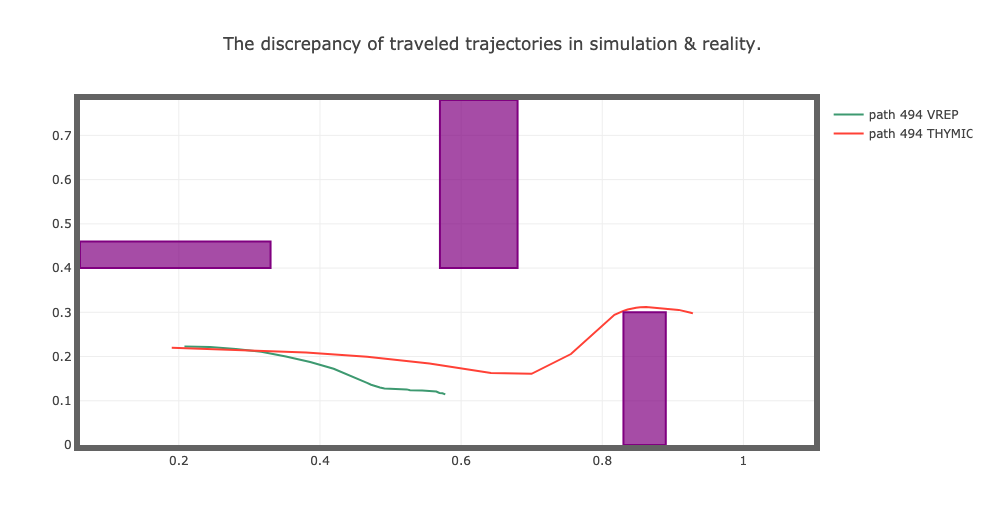
\includegraphics[width=5cm]{include/images/trajectory_discrepancy.PNG}
        \caption{The discrepancy of traveled trajectories in simulation and reality.}
        \label{fig:trajectory_discrepancy}
    \end{subfigure}
    \begin{subfigure}[b]{0.8\textwidth}
    	\centering
        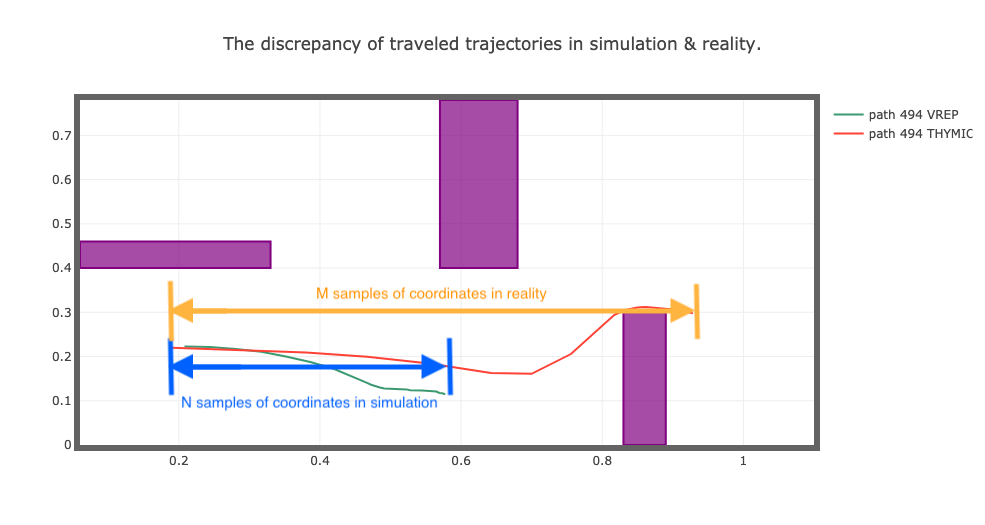
\includegraphics[width=5cm]{include/images/trajectory_discrepancy_wrong_measure.PNG}
        \caption{Potential miscalculations of the exact STR Disparity.}
        \label{fig:trajectory_discrepancy_wrong_measure}
    \end{subfigure}
    % \caption{Reality-based simulation results I.}
	\label{fig:real_based_resultsI}
\end{figure}

\item{Defects in Thymio Robot}.

\item{Diversity & Surrogate Model}.

\section{Results}

The table \ref{tab:summary_experiments} sums up the experiments taken in simulation, reality or both when concerning the transferability approach. It also summarizes the number of evaluations on the physical robot for each approach along the time it took to run. The simulation-based and reality-based approaches have been implemented using the NEAT algorithm, while the transferability approach was implemented using the NSGA algorithm. Each approach was reproduced 10 times except for the transferability approach. Following the results section, we define an optimal solution as a controller that solves the task, meaning a controller that is able to avoid obstacles.


\begin{table}[ht]
\resizebox{\textwidth}{!}{%
\begin{tabular}{@{}|l|cc|l|l|l|l|@{}}
\toprule
\multicolumn{1}{|c|}{\multirow{2}{*}{\textbf{Approach}}} & \multicolumn{2}{c}{\textbf{Evaluation}} & \multirow{2}{*}{\textbf{\begin{tabular}[c]{@{}l@{}}Number of \\ simulation runs\end{tabular}}} & \multirow{2}{*}{\textbf{\begin{tabular}[c]{@{}l@{}}Number of evaluations\\ on the physical robot\end{tabular}}} & \multirow{2}{*}{\textbf{\begin{tabular}[c]{@{}l@{}}Evolutionary\\ Algorithm\end{tabular}}} & \multirow{2}{*}{\textbf{\begin{tabular}[c]{@{}l@{}}Average\\ running time	\end{tabular}}} \\ \cmidrule(lr){2-3}
\multicolumn{1}{|c|}{} & \multicolumn{1}{c|}{\textit{Simulation}} & \textit{Reality} &  &  &  &  \\ \midrule
Simulation based app. & \multicolumn{1}{c|}{X} &  & 10 & 0 & NEAT & $\sim$4 hours \\ \midrule
Reality based app. & \multicolumn{1}{c|}{} & X & 10 & 4000 & NEAT & $\sim$18 hours \\ \midrule
Transferability app. & \multicolumn{1}{c|}{X} & X & 5 & 236 (average) & MOEA & $\sim$6 hours \\ \bottomrule
\end{tabular}%
}
\caption{Evaluations taken place in simulation, reality or both.}
\label{tab:summary_experiments}
\end{table}

\subsection{Results for the simulation-based optimization}

Figure \ref{fig:sim_avg_fitness} shows the average fitness performance of 10 simulation runs in simulation. The optimality of any given controller is hard to determine since the fitness is simply maximized. However, it is clear from the figure that the fitness is progressing towards some optimum. Furthermore, figure \ref{fig:sim_best_genomes_percentile} shows the performance of the best genomes in each generation across all simulation runs. In addition, it shows the median and 25\%/75\% percentiles. The smooth max curve in some generations is the evidence of elitism in the NEAT algorithm set up. 

\begin{figure}[H]
    \centering
    \begin{subfigure}[b]{0.8\textwidth}
    	\centering
        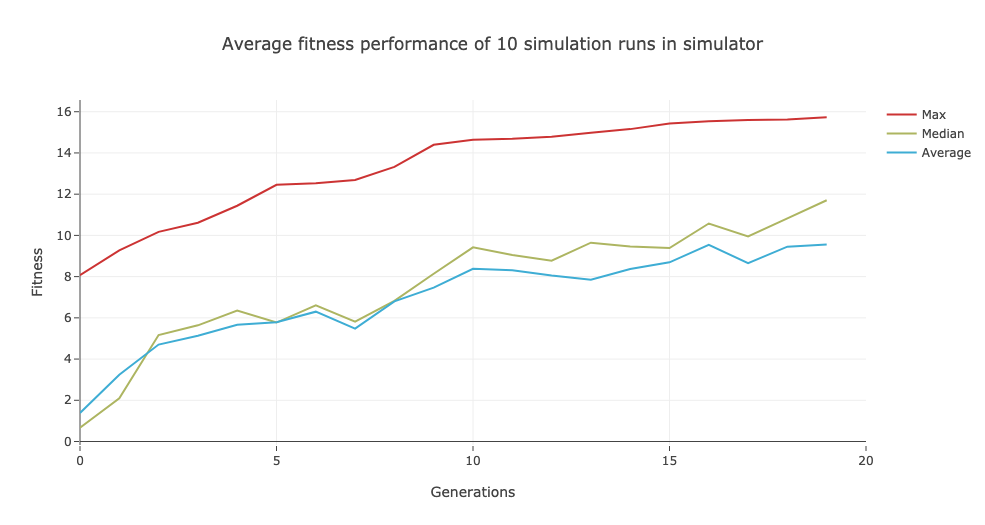
\includegraphics[width=5cm]{include/images/sim_avg_fitness.PNG}
        \caption{Average fitness of 10 simulation runs}
        \label{fig:sim_avg_fitness}
    \end{subfigure}
    \begin{subfigure}[b]{0.8\textwidth}
    	\centering
        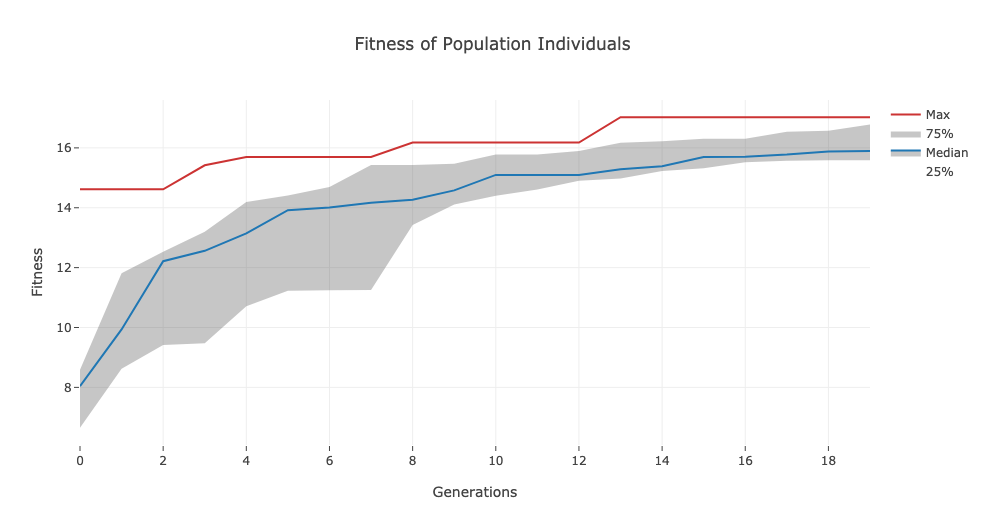
\includegraphics[width=5cm]{include/images/sim_best_genomes_percentile.PNG}
        \caption{Best controllers each generation over all the runs.}
        \label{fig:sim_best_genomes_percentile}
    \end{subfigure}
    \caption{Simulation based results I.}
	\label{fig:sim_based_resultsI}
\end{figure}

Figure \ref{fig:sim_fitness_distribution} shows the distribution of each individual in the population for a single simulation run. Each evolutionary run took on average \~4 hours, thus \~40 hours in total. The objective was to evolve controllers that exhibit obstacle avoidance behavior. The visual manifestation of behaviors is depicted in figure \ref{fig:sim_path_travelled}. It shows the path taken by the best genomes in each simulation run. It is noticeable that each controller moves forward until it makes a sharp turn to the left to avoid a collision with an obstacle. To further validate the robustness of best controllers, the obstacles in the simulation where randomly misplaced from their initial positions, and each genome was post-evaluated in a slightly new environmental set-up. Again all the genomes exhibited the desired obstacle avoidance behavior. This showcase that the evolved controllers are able to generalize.

\begin{figure}[H]
    \centering
    \begin{subfigure}[b]{0.8\textwidth}
    	\centering
        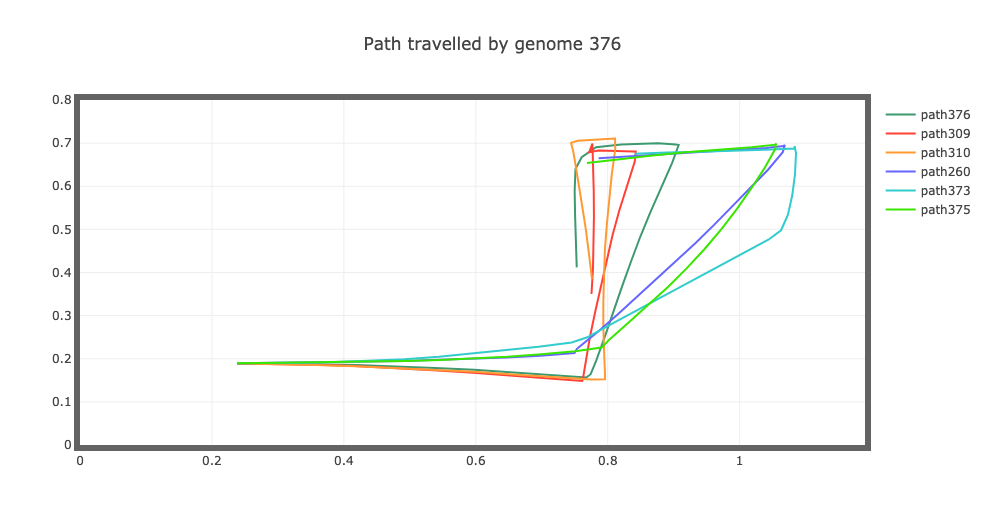
\includegraphics[width=8cm]{include/images/sim_path_travelled.PNG}
        \caption{Path travelled by the best genomes.}
        \label{fig:sim_path_travelled}
    \end{subfigure}
    \begin{subfigure}[b]{0.8\textwidth}
    	\centering
        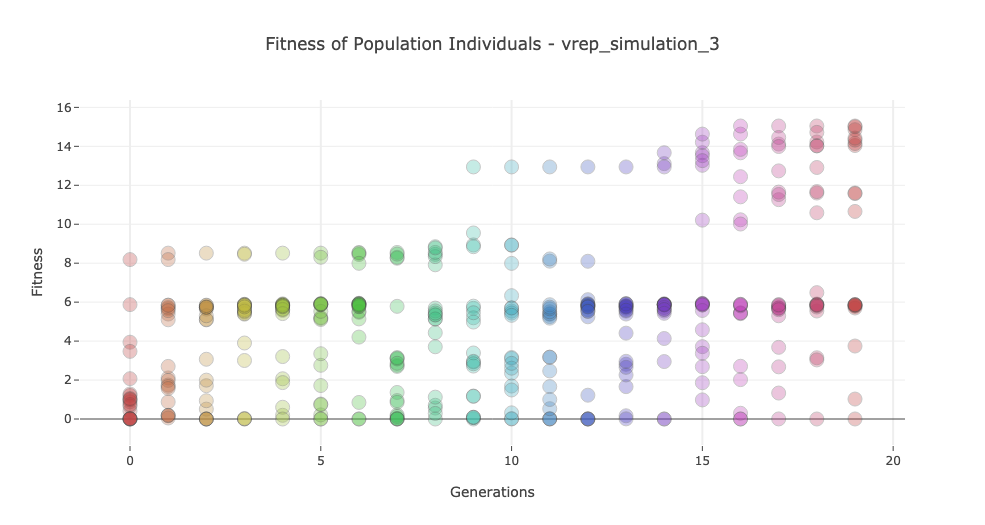
\includegraphics[width=8cm]{include/images/sim_fitness_distribution.PNG}
        \caption{Fitness distribution of population individuals for a single run.}
        \label{fig:sim_fitness_distribution}
    \end{subfigure}
    \caption{Simulation based results II.}
	\label{fig:sim_based_resultsII}
\end{figure}

Another interesting result concerns the behavioral features of the best genomes. As can be seen in figure \ref{fig:sim_behavioral_features_best}, it appears that all the genomes have almost the same behavioral values. The average wheel speed values indicates that the robots right wheel is set at full speed at evaluation while the right motor is not. This explains while the robot takes always left turns. Since the left motor is set to lower values than the right motor. Additionally, the front horizontal sensors (s1-s5) are the most active, while the back sensors (s6 and s7) are least active.

\begin{figure}[H]
    \centering
    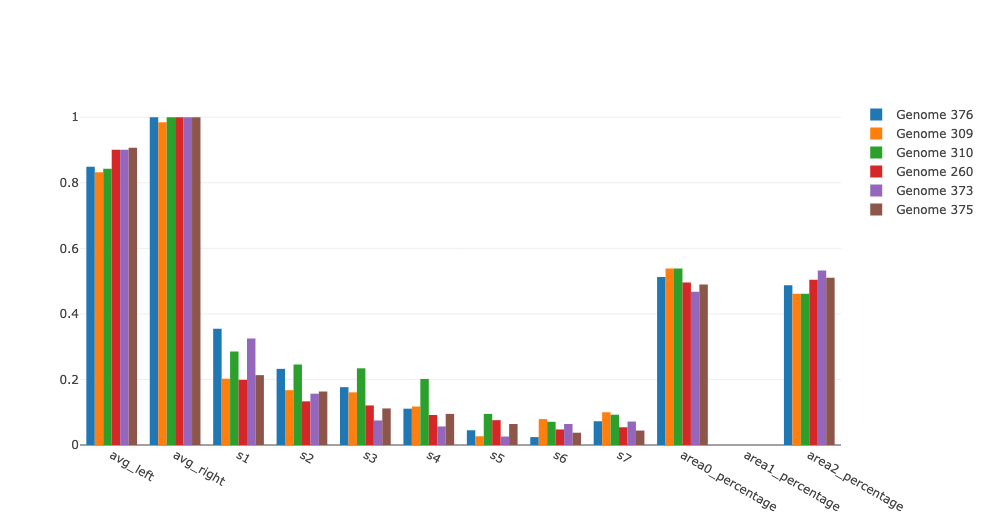
\includegraphics[width=8cm]{include/images/sim_behavioral_features_best.PNG}
    \caption{Behavioral features of the best genomes.}
    \label{fig:sim_behavioral_features_best}
\end{figure}

\begin{table}[h]
\centering
\begin{tabular}{ccc}
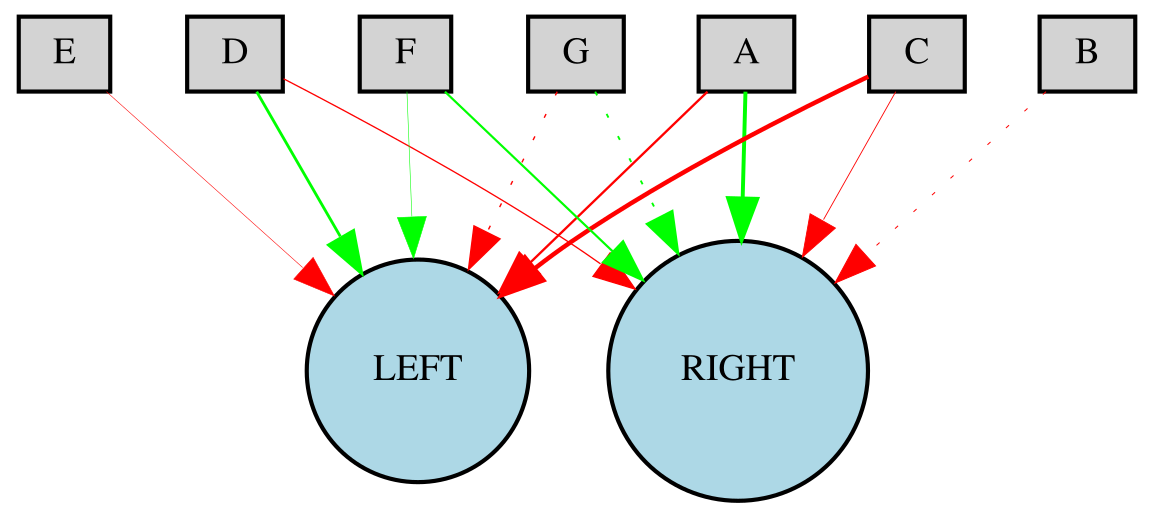
\includegraphics[scale=0.4]{include/images/sim_network_1.PNG} & 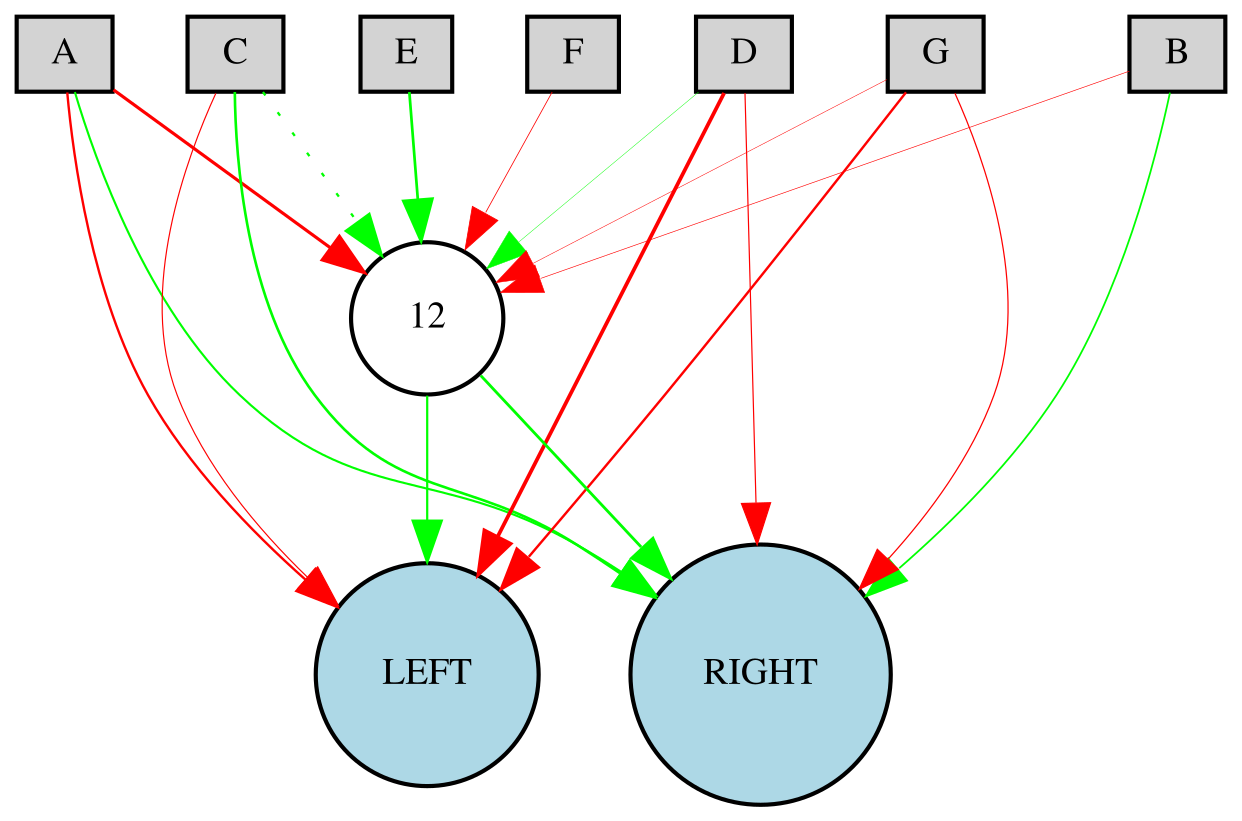
\includegraphics[scale=0.4]{include/images/sim_network_2.PNG} & 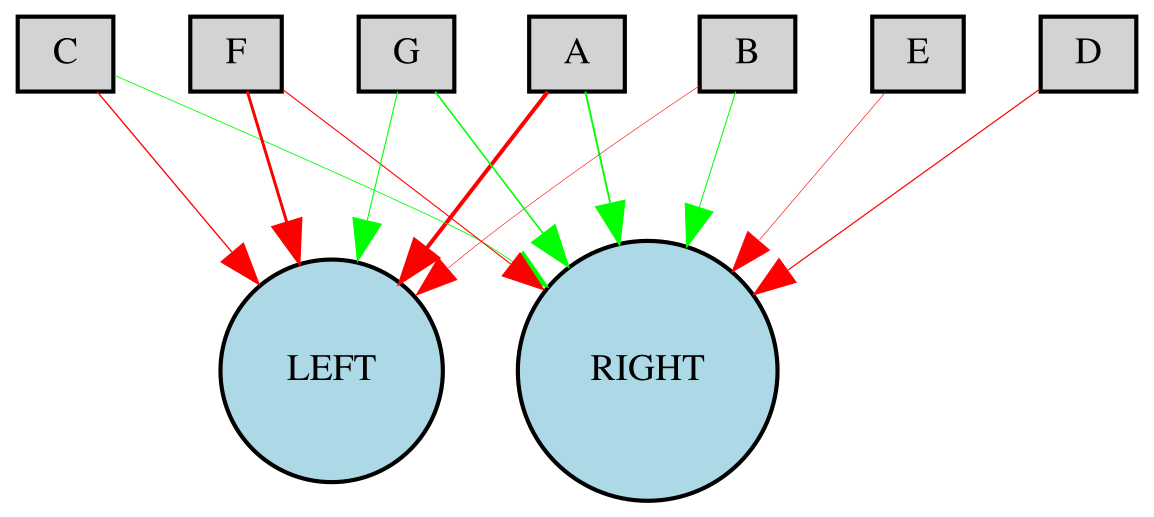
\includegraphics[scale=0.4]{include/images/sim_network_3.PNG} \\
$$Genome \;  \; 376$$  & $$Genome \;  \; 309$$  & $Genome \;  \; 310$  \\
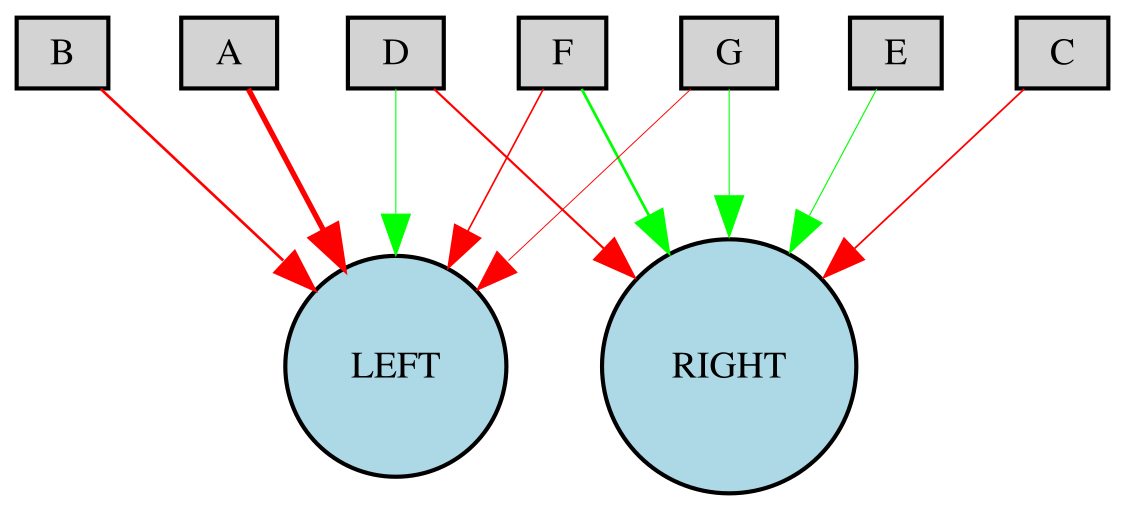
\includegraphics[scale=0.4]{include/images/sim_network_4.PNG} & 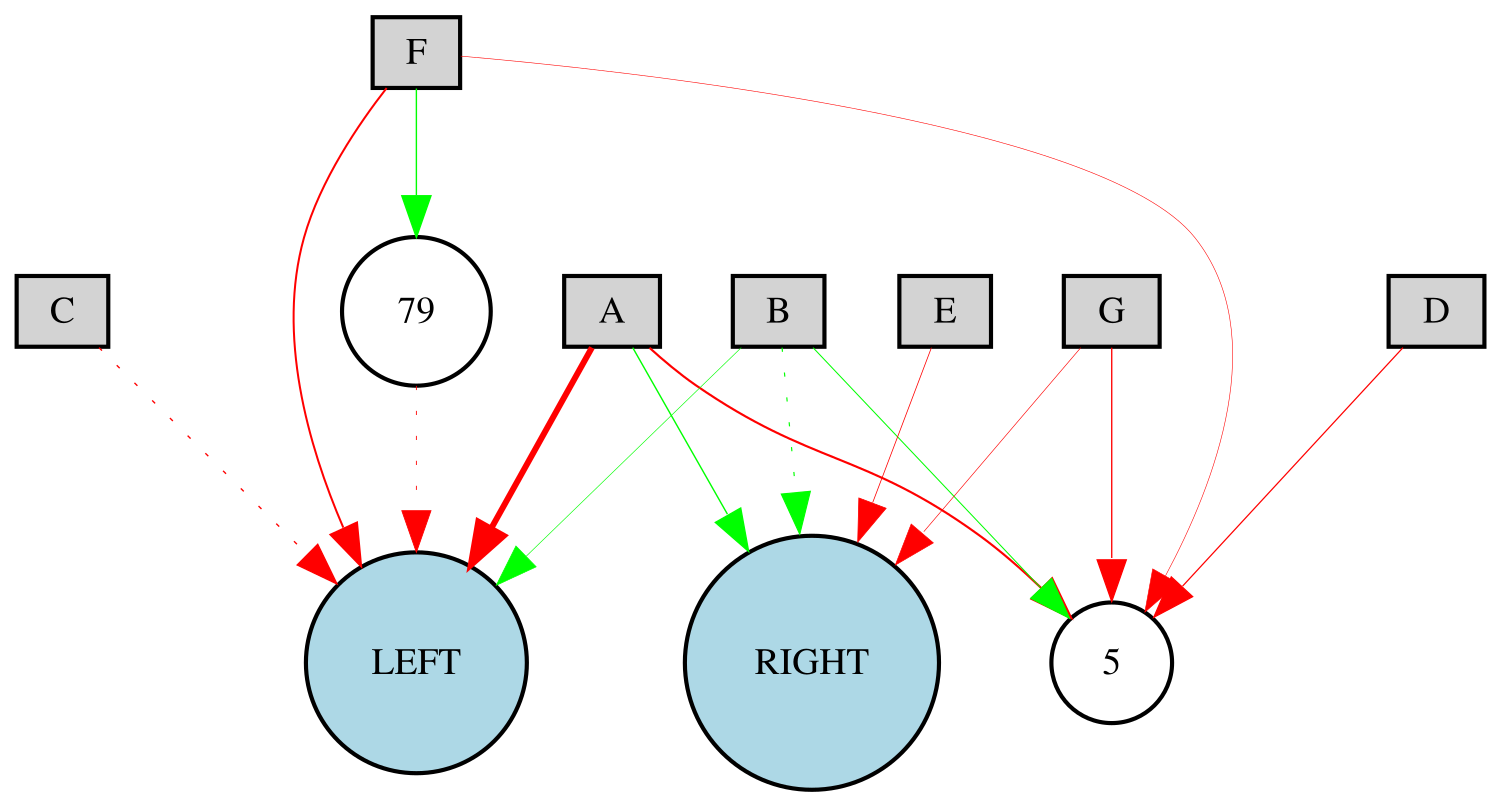
\includegraphics[scale=0.4]{include/images/sim_network_5.PNG} & 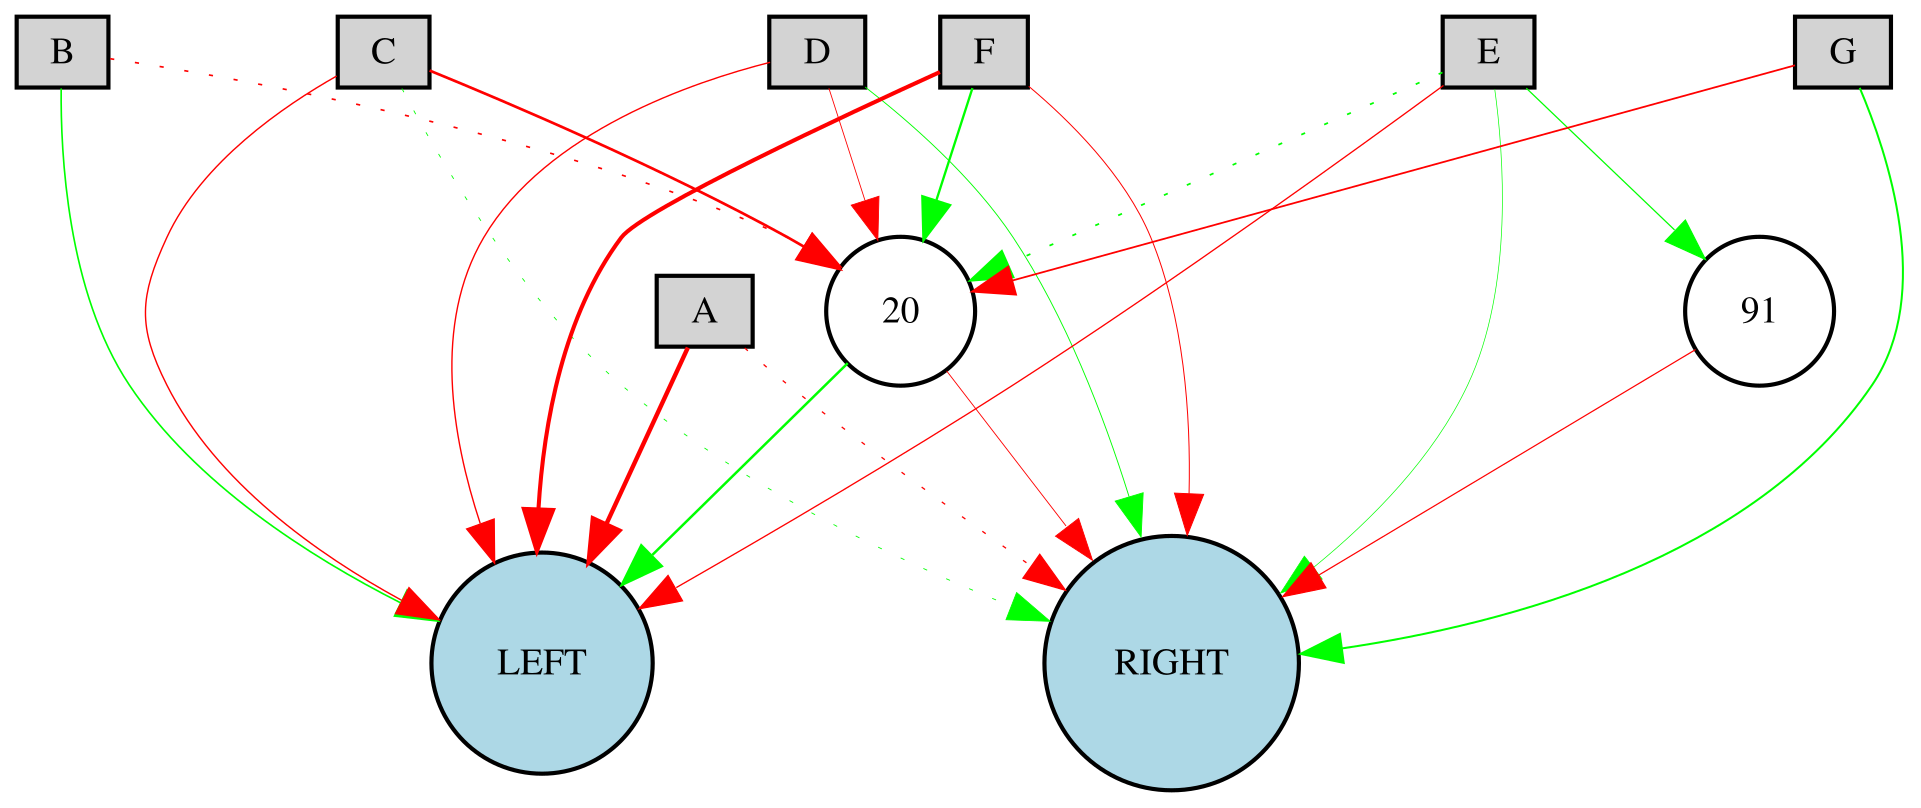
\includegraphics[scale=0.4]{include/images/sim_network_6.PNG} \\
$Genome \;  \; 260$  & $Genome \;  \; 373$  & $Genome \;  \; 375$  \\
\end{tabular}
\caption{Evolved topology of the best controllers in simulation.}
\label{fig:sim_network_topologies} % 
\end{table}

The evolved topologies of the neural networks can be seen in figure \ref{fig:sim_network_topologies}. The green and red color connections represent positive/negative weight values. Notice that not all the connections are enabled. The doted connections refer to connections that were disabled over time. In addition, the evolutionary process has evolved a hidden layer with 1 or 2 neurons in some cases (Genome 375, Genome 373 or Genome 309).

\emph{Transferability.} To validate and examine whether the evolved controllers in a simulation are transferable we took the best controllers from each simulation run and transferred them directly to the Thymio robot. For example, a behavior of the best controller transferred to reality is depicted in figure \ref{fig:sim_bad_transfer}. The trajectory of the controller in the simulator is shown with a dark green color. The transferred controller is post evaluated 10 times and its typical behavior consists of going straight without taking into account the obstacle in front. Among one of them (red) attempts to avoid the obstacle, however unsuccessfully as it afterward turns to directly to the obstacle and keeps colliding with it. It undoubtedly highlights that there is a reality-gap problem between simulation and reality. However, as it turned out this gap can be convoluted. Among the transfered controllers (10), we have identified 2 controllers that are transferable and able to avoid obstacles. A typical behavior of a transferable controller is picture on \ref{fig:sim_good_transfer}. This lead to a conclusion that there is a clear gap between simulation and reality, however, sometimes good solutions can be evolved in simulators that are transferable to reality.

\begin{figure}[H]
    \centering
    \begin{subfigure}[b]{0.8\textwidth}
    	\centering
        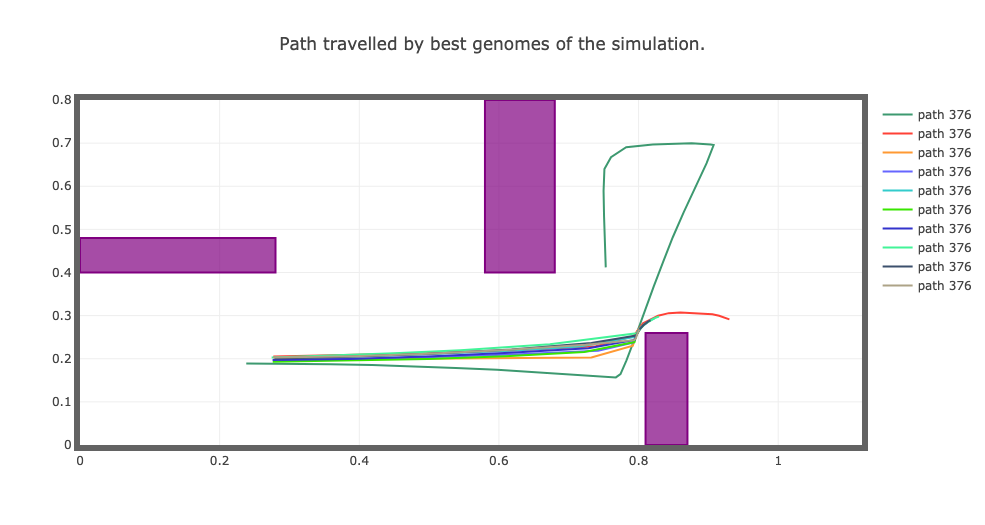
\includegraphics[width=8cm]{include/images/sim_bad_transfer.PNG}
        \caption{Controller that is not transferable.}
        \label{fig:sim_bad_transfer}
    \end{subfigure}
    \begin{subfigure}[b]{0.8\textwidth}
    	\centering
        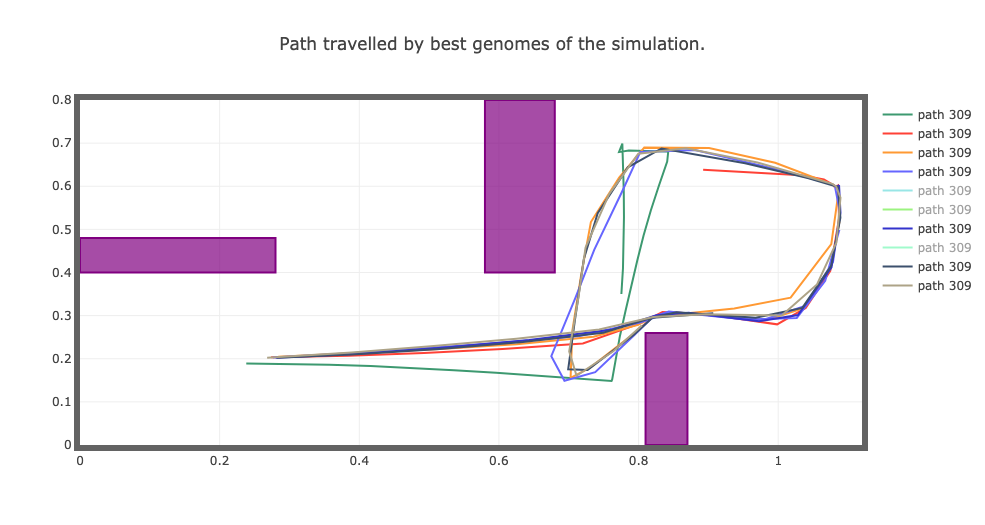
\includegraphics[width=8cm]{include/images/sim_good_transfer.PNG}
        \caption{Controller that transfered well to reality.}
        \label{fig:sim_good_transfer}
    \end{subfigure}
    \caption{Typical behaviors of the best controllers transferred to reality. Each of them post-evaluated 10 times in reality.}
	\label{fig:transferred_controllers}
\end{figure}

\subsection{Results for the reality-based optimization}

The summary of results are depicted in figure \ref{fig:real_based_resultsI}. The thymio evolved an obstacle avoidance behavior in less than 20 generations. Each simulation run taking  approximately 16 hours, thus 160 hours in total. Most of the best thymio controllers maintain a straight trajectory and perform right turns when necessaary. Like in the previous experiment, there is no clear way to differentiate between optimal solutions and non-optimal ones from the fitness, it is simply maximized. Looking at the figure \ref{fig:real_best_genomes_percentile} of the best controllers, it indicates that controllers with high fitness emerge by the 10th generation, even though the progress is not smooth as in the simulation-based optmization. However, the dips in the curves are the result of noise. Figure \ref{fig:thymio_network_topologies} shows the evolved topologies of the best 6 controllers.

\begin{figure}[H]
    \centering
    \begin{subfigure}[b]{0.8\textwidth}
    	\centering
        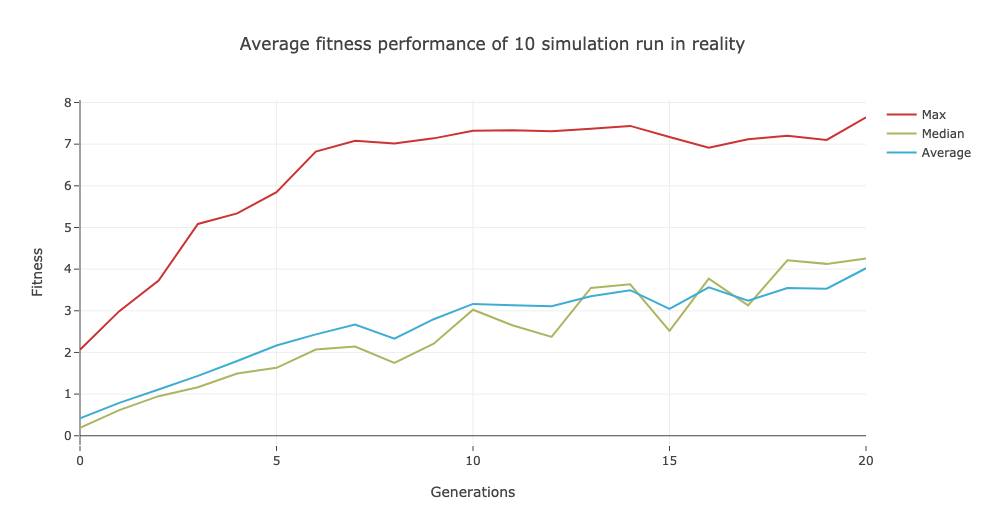
\includegraphics[width=5cm]{include/images/real_avg_fitness.PNG}
        \caption{Average fitness of 10 simulation runs.}
        \label{fig:real_avg_fitness}
    \end{subfigure}
    \begin{subfigure}[b]{0.8\textwidth}
    	\centering
        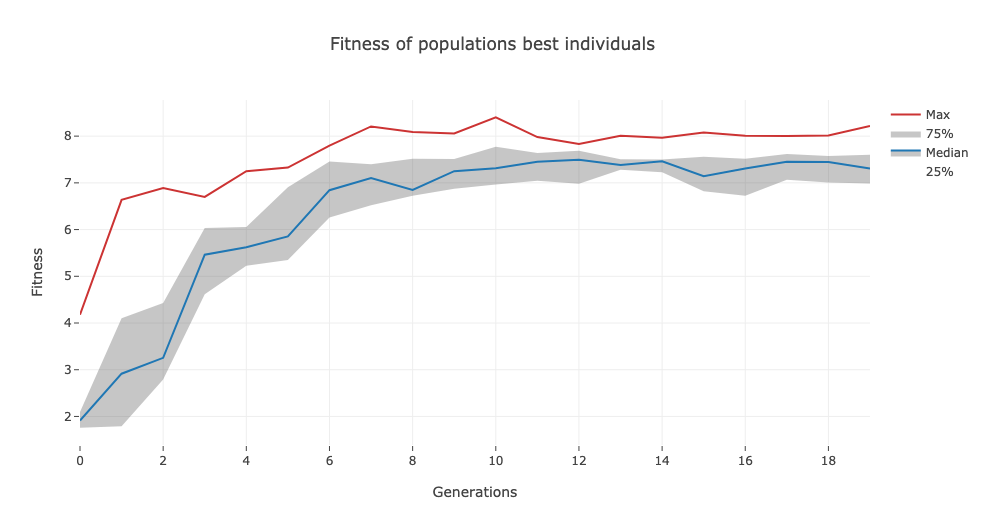
\includegraphics[width=5cm]{include/images/real_best_genomes_percentile.PNG}
        \caption{Best controllers each generation over all the runs.}
        \label{fig:real_best_genomes_percentile}
    \end{subfigure}
    \caption{Reality-based simulation results I.}
	\label{fig:real_based_resultsI}
\end{figure}

The corresponding behavior of 5 best controllers is depicted in figure \ref{fig:path_traveled_thymio_reality_based}. 2 of them have similar behavior, going straight and making a sharp \emph{U} turn after they sense the obstacle in front of them. On the other hand \emph{Genomes 189, 73, 24}, are taking a left turn and keep moving around in the the second area most of the time.


\begin{table}[h]
\centering
\begin{tabular}{ccc}
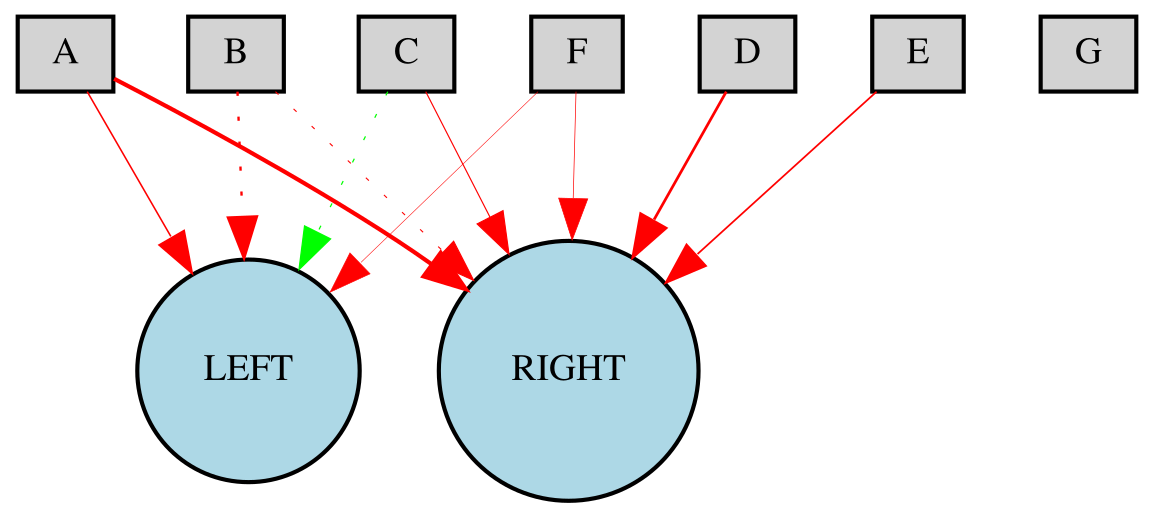
\includegraphics[scale=0.4]{include/images/thymio_network_379.PNG} & 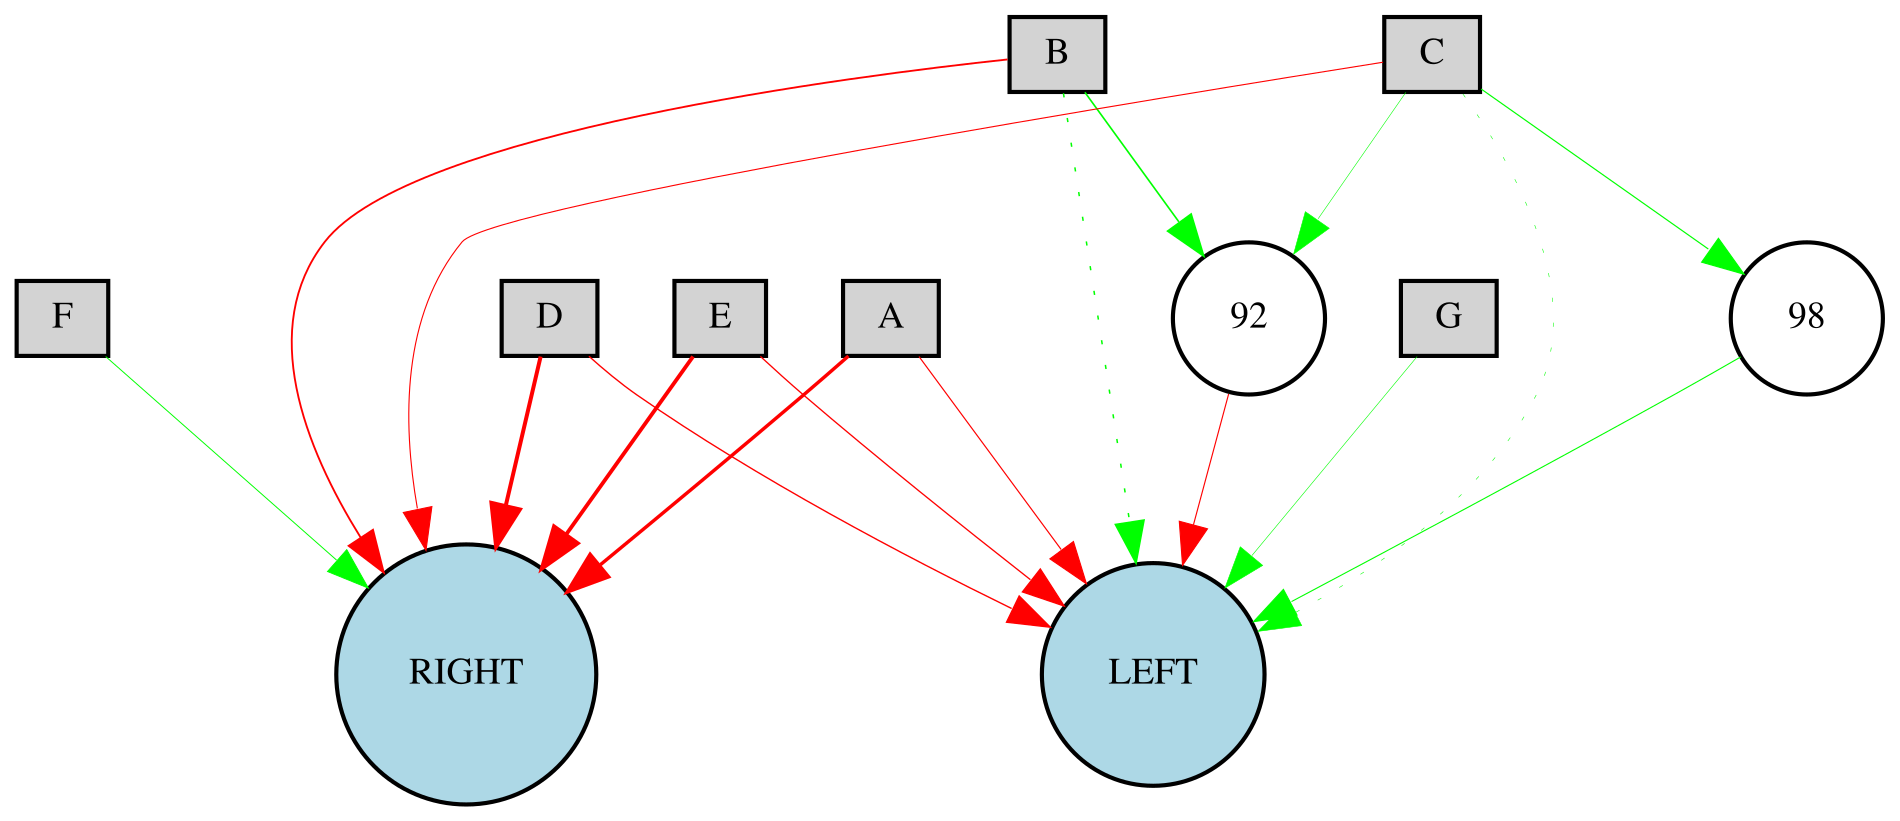
\includegraphics[scale=0.4]{include/images/thymio_network_78.PNG} & 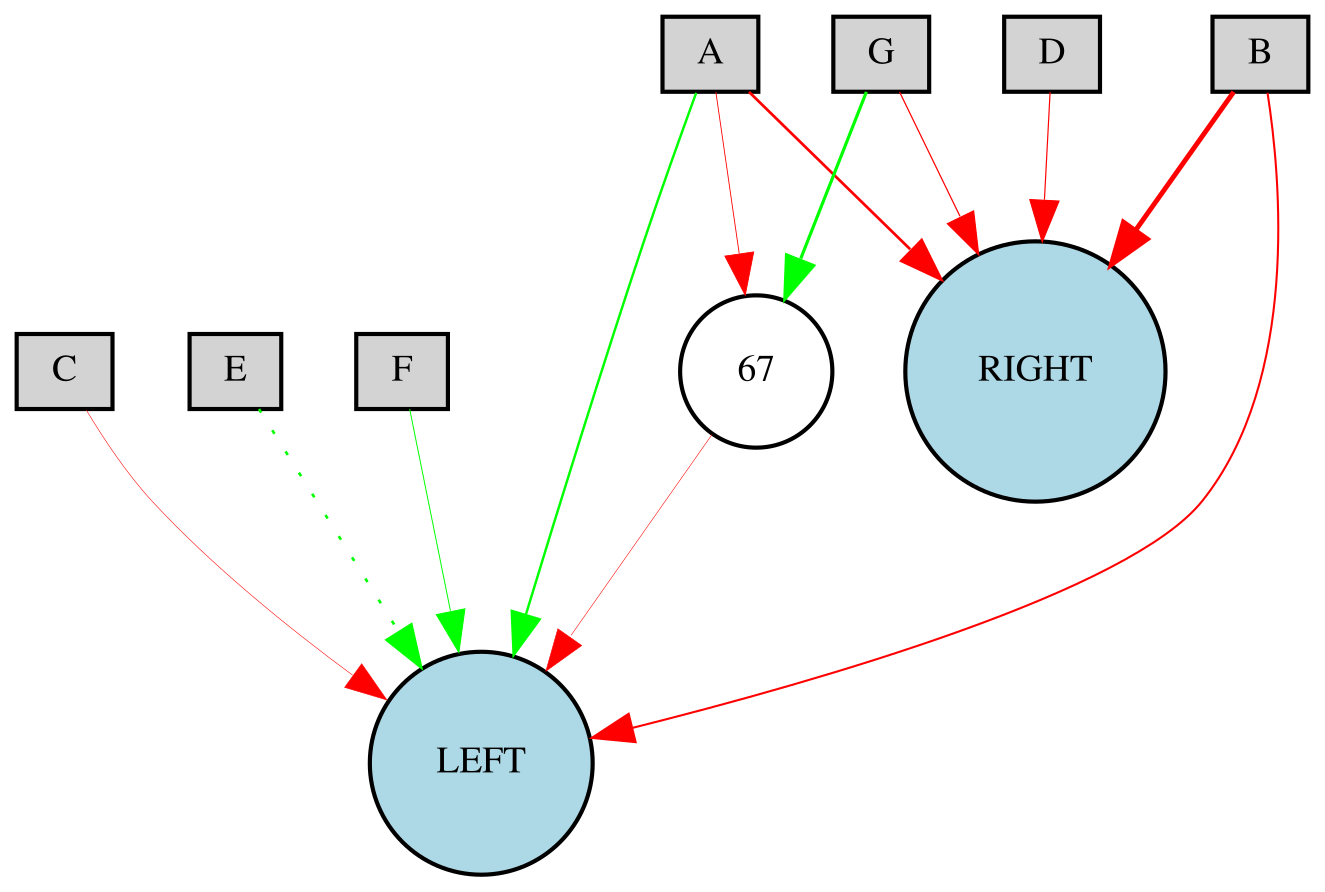
\includegraphics[scale=0.4]{include/images/thymio_network_73.PNG} \\
$$Genome \;  \; 379$$  & $$Genome \;  \; 78$$  & $Genome \;  \; 73$  \\
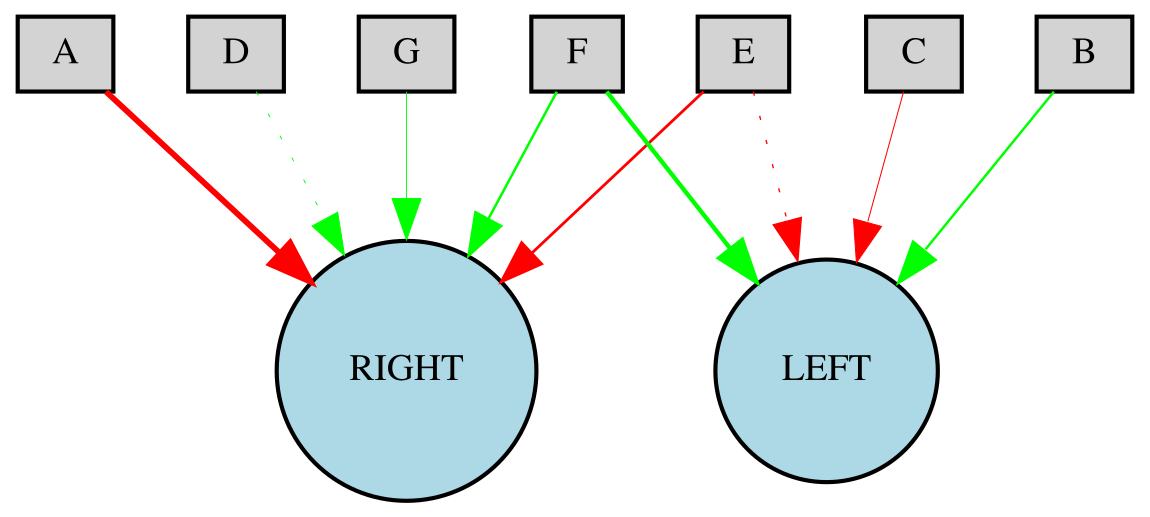
\includegraphics[scale=0.4]{include/images/thymio_network_343.PNG} & 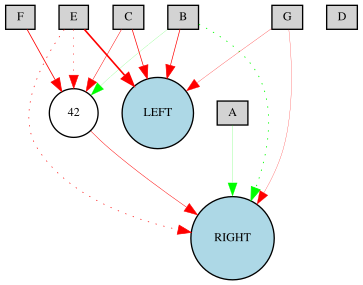
\includegraphics[scale=0.4]{include/images/thymio_network_50.PNG} & 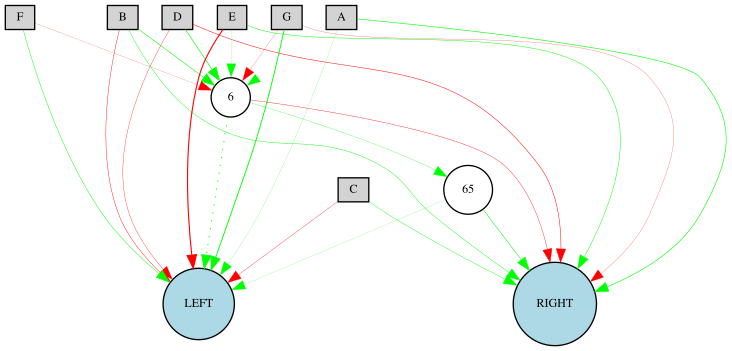
\includegraphics[scale=0.4]{include/images/thymio_network_189.PNG} \\
$Genome \;  \; 343$  & $Genome \;  \; 50$  & $Genome \;  \; 189$  \\
\end{tabular}
\caption{Evolved topology of the best controllers in reality.}
\label{fig:thymio_network_topologies} % 
\end{table}

\subsection{Results with the Transferability approach}

The transferability approach with the heuristic update function based on the fitness threshold criteria works well for all the 5 runs. At the end of the multi-objective evolutionary run, we obtain on average a set of 5 non-dominated solutions. On average the best solutions achieve \textit{10.65} fitness value. A typical fitness landscape obtained with transferability approach is depicted in figure \ref{fig:best_pareto}. It shows the 2 parameters that are optimized along with the non-dominated solutions on the Pareto front.

\begin{figure}[H]
	\centering
  	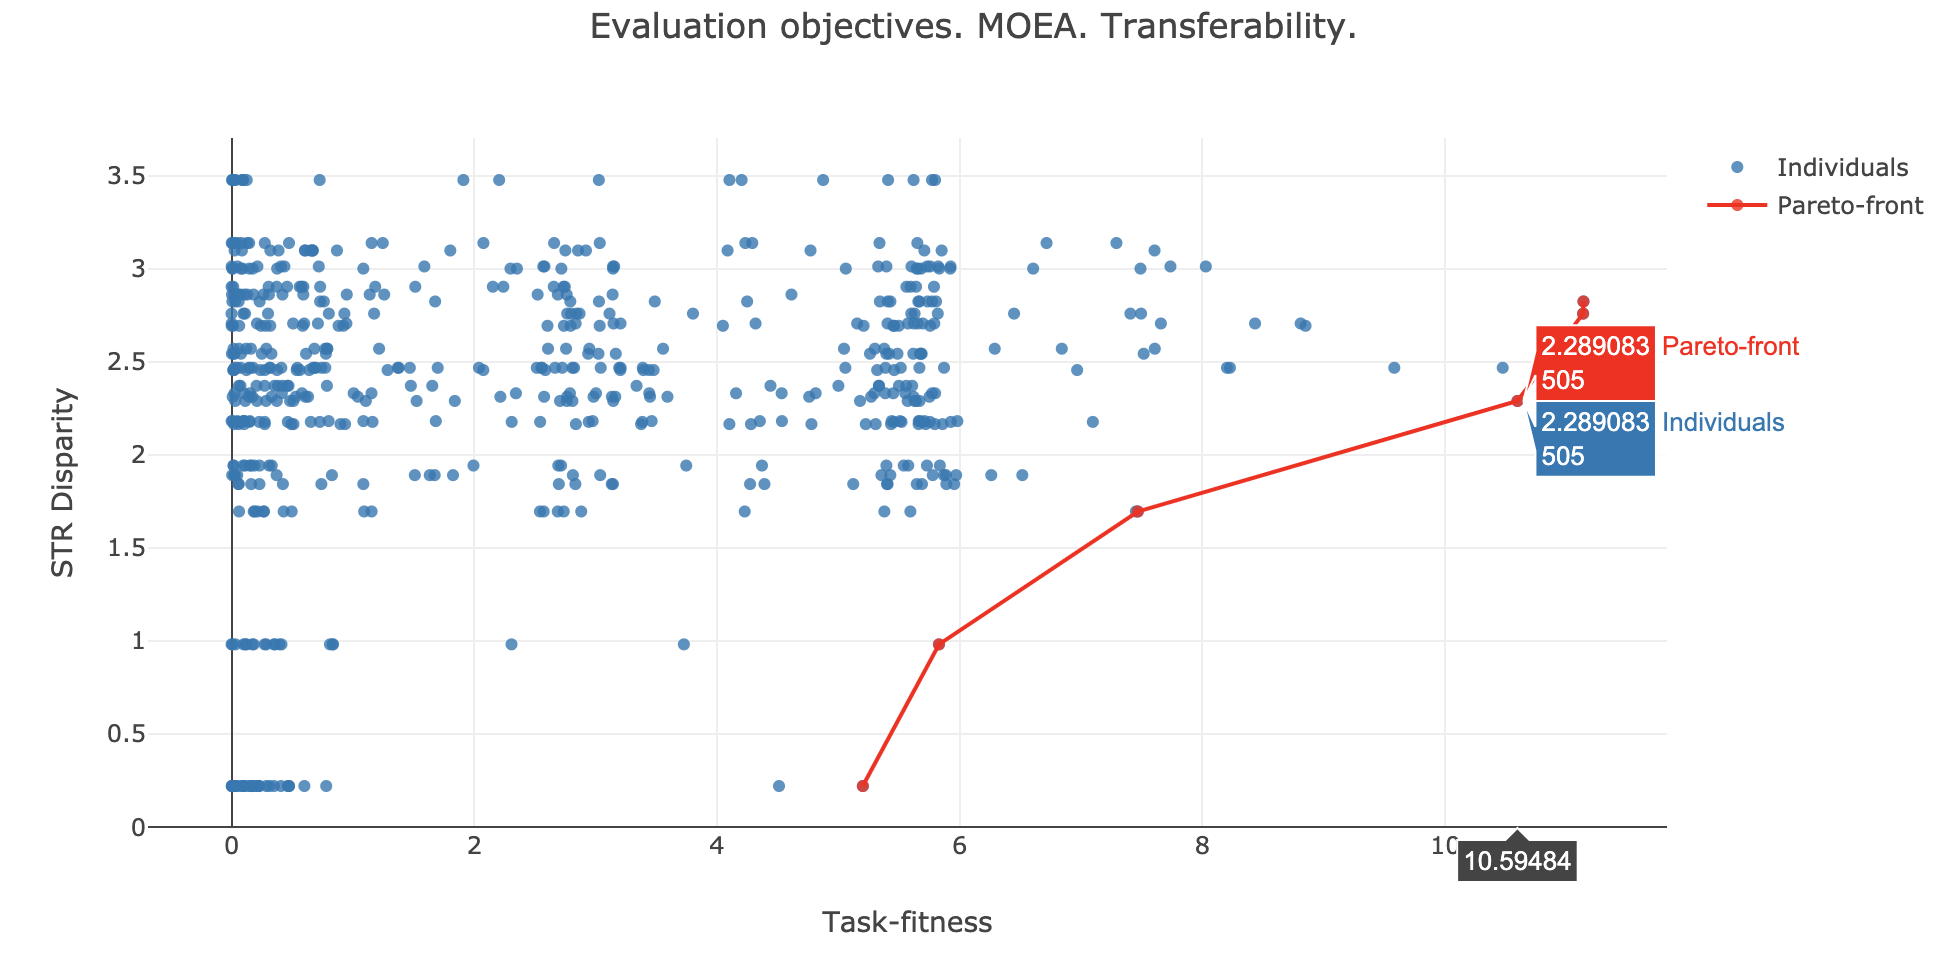
\includegraphics[width=6cm]{include/images/pareto_best_moea.PNG}
  	\caption{A typical fitness landscape obtained with transferability approach.}
  	\label{fig:best_pareto}
\end{figure}

Altought the non-dominated set contains the best solutions of the run, in some cases the most efficient solutions (solutions with the highest fitness) in simulation are not transferable to the physical  robot. Therefore we have to choose the best compromise between efficiency and transferability in this set. This is showcased in figure \ref{fig:comparison_efficiency_transferability}. Controller \textit{594} with the highest fitness value of \texit{11.13} and approximated disparity of \texit{2.82} is the most efficient from the entire population but not transferable. On the other hand controller \textit{505} with lower fitness value of \textit{10.59} and approximated STR diparity value of \textit{2.28} is at the same time optimal in reality (avoids obstacles) and transferable.

\begin{figure}[H]
    \centering
    \begin{subfigure}[b]{0.8\textwidth}
    	\centering
        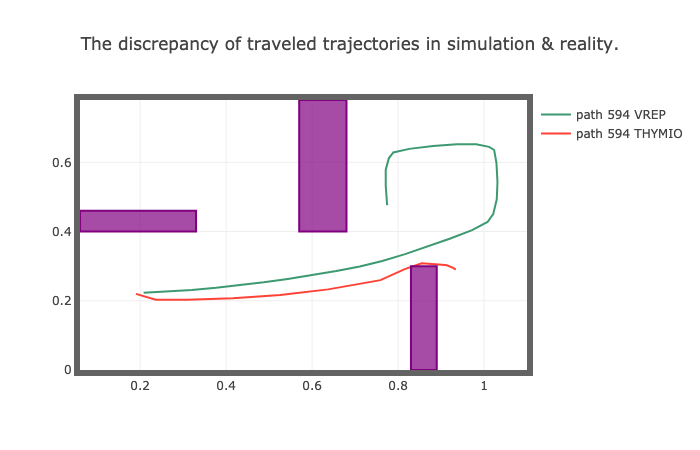
\includegraphics[width=8cm]{include/images/fit_not_transferable.PNG}
        \caption{Controller with the highest fitness from a simulation run.}
        \label{fig:sim_bad_transfer}
    \end{subfigure}
    \begin{subfigure}[b]{0.8\textwidth}
    	\centering
        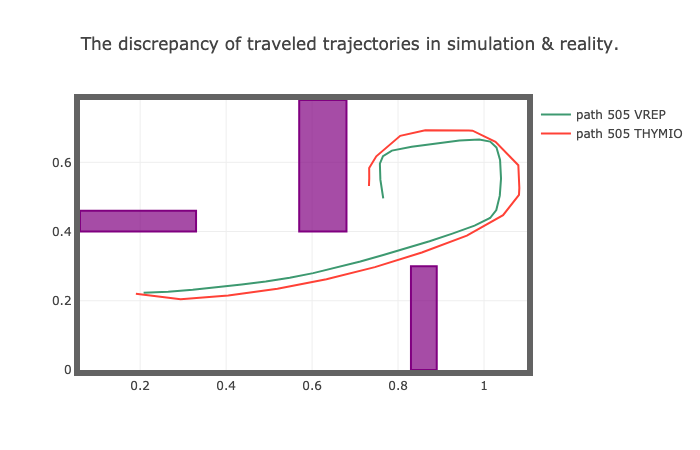
\includegraphics[width=8cm]{include/images/moea_sim_18_505.PNG}
        \caption{Controller that is less efficient but transferable.}
        \label{fig:sim_good_transfer}
    \end{subfigure}
    \caption{Comparison between efficiency and transferability.}
	\label{fig:comparison_efficiency_transferability}
\end{figure}

\subsection{Summary of the results}

The fitness of the best solutions found with all approaches can be seen in figure \ref{fig:fitness_comparison}. Means and quartiles are computed on 10 runs, except for the transferability approach with 5 runs. Although the transferability approach has lower fitness values than the simulation-based approach, it clearly behaves the best and always find solutions that are both optimal in reality and transferable. Even though, sometimes using advanced simulation tools might lead to transferable controllers that perform efficiently. The lower fitness values of the transferability approach might be the cause of the different evolutionary algorithm utilized. Since the NEAT algorithm has the advantage of evolving both the topology and the weights of the artificial neural network, moreover the network weights values are initialized by the algorithm itself. This in contrast to MOEA where we had to construct explicitly the topology of the neural network, initialize and encode every connection weights as a list of floating points numbers to represent the genomes would require more evaluations to explore efficiently the solution space. As it was also the case in the preliminary experiments, where we had to extend the number of generations from 20 to 30 in order to evolve obstacle avoidance behavior with MOEA. Compared to the reality-based optimization approach, the transferability approach behaves better, considering also the time to evolve the given behavior which is 3x less time-consuming.

\begin{figure}[H]
	\centering
  	\includegraphics[width=9cm]{include/images/fig:fitness_comparison.PNG}
  	\caption{Fitness of the best solutions found with all the approaches.}
  	\label{fig:best_pareto}
\end{figure}

\section{Furthere Discusion on the Transferability approach}

As described in the section \emph{Complications of the implementation}, in the initial experiments we transferred controllers based on a diversity threshold of 0.5, that corresponded to an average of 80 transfer by run (5 runs in total). Within this selection criteria, we have obtained a surrogate model with a larger error. Despite the lack of time, we have decided to change the selection criteria based on a fitness threshold. To determine if the surrogate model is more accurate with the fitness threshold approach we compared the approximated STR disparity values to the exact STR disparity values. Figure \ref{fig:str_disparities} shows the corresponding approximated STR disparity values and the exact STR disparity values of all the non-dominated solutions from the Pareto-Front for each run. Figure \ref{fig:bad_str_disparity} corresponds to disparity values obtained with diversity threshold 0.5, while figure \ref{fig:good_str_disparity} corresponds disparity values obtained with the fitness threshold 3.0.

\begin{figure}[H]
    \centering
    \begin{subfigure}[b]{0.8\textwidth}
    	\centering
        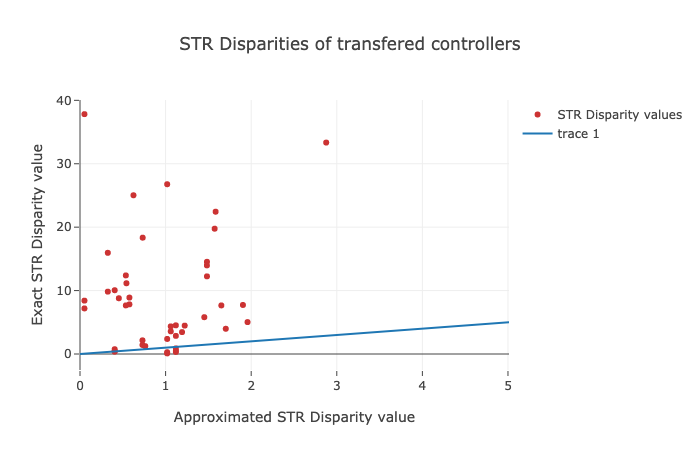
\includegraphics[width=5cm]{include/images/moea_worst_hofs.PNG}
        \caption{Results with the diversity threshold.}
        \label{fig:bad_str_disparity}
    \end{subfigure}
    \begin{subfigure}[b]{0.8\textwidth}
    	\centering
        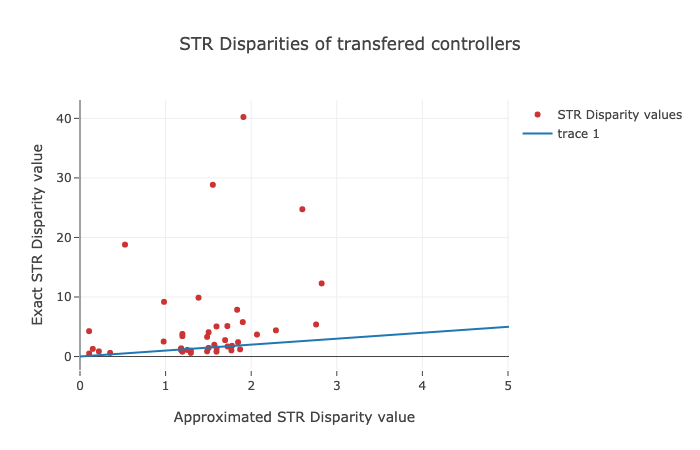
\includegraphics[width=5cm]{include/images/moea_best_hofs.PNG}
        \caption{Results with the fitness threshold.}
        \label{fig:good_str_disparity}
    \end{subfigure}
    \caption{Approximated STR disparity compared to exact STR disparity for all the non-dominated solutions in the Pareto-front obtained with the diversity & fitness threshold selection approach.}
	\label{fig:str_disparities}
\end{figure}

In general, the surrogate models of the approximated STR disparity tends to underestimate the exact values for very high disparity values. However, this is the side effect of the Inverse Distance Weighing interpolation technique, which is highly sensitive to outliers. According to figure \ref{fig:str_disparities} it is clear that the surrogate model obtained with the fitness threshold selection criteria is better at approximating the exact STR disparities. When computing the mean square error between the approximated STR disparity and the exact STR disparity, we obtain \textit{79.128} with the fitness selection method and \textit{143.951} with the diversity selection method for 43 individuals from the Pareto front and 44 individuals. Even though the mean square error values are high in both cases, which is the result of heavily weighting large errors of the function, we can conclude that the surrogate model is of better quality with the fitness selection method. From our observation, we assume that the main reason for the higher error of the surrogate model using the diversity selection method is caused by choosing the inappropriate behavioral features and behavioral distances calculation.

In the early stages of the experiments, the update heuristic function that selects which controllers to transfer to the physical robot consisted of choosing controllers whose diversity values are greater than the specified diversity threshold of \textit{0.5}. Compared to the heuristic function that chooses controllers to transfer among whose fitness value is greater than \textit{3.0} we have obtained less accurate surrogate model and less transferable individuals. We hypothesize, that the poor results obtained with this heuristic function are caused by choosing the inappropriate behavioral features for the diversity measure. The behavioral distance measure is computed as the Euclidean distance based on the controllers' 12th behavioral features \ref{eq:behavioral_features} to the already transferred controller's behavioral features. The diversity corresponds to taking the minimal behavioral distance between the specific controller and the already transferred controllers. This feature-based behavioral distance appeared to be too diverse as the behavioral features consist mostly of sensory readings. We believe that determining the diversity of a controller on such sparse information is not precise enough to build an accurate surrogate model. An effective behavioral-distance measure certainly has to determine the different type of behaviors observed in simulation. For instance, in our application, instead of relying on the sensors features other behaviors like the traveled distance, the orientation of the robot, distance between the various obstacle could have been more efficient to determine the diversity of the controllers.



